\chapter{集合} \label{chap:set}

集合是高中数学接触到的第一个概念,也是数学领域最基础的数学概念之一。在本章中,我
们将拓展一些高中内容。本章的后半部分还使用大量篇幅介绍了集合基数相关知识,其与高
中内容联系有限,仅供读者拓展知识。

\section{超集、相对补集}

我们在高中已经学习到了一些和集合相关的内容。我们知道元素和集合间的关系:
\textbf{属于};知道集合和集合间的关系:\textbf{包含于};知道集合间的运算:
\textbf{交集}、\textbf{并集}和\textbf{补集}。

我们知道,关系是相互的——小王是老王的儿子,老王是小王的父亲;那放之于集合的范畴,
我们定义了和子集相对的概念——超集:

\begin{rawdef}[超集]\index{超集}
    集合$A$的\textbf{超集}$B$是一个集合,它含有$A$中的所有元素。记作$B \supseteq 
    A$.
\end{rawdef}

也就是说,如果$B$包含$A$,那$B$就是$A$的一个超集。这个概念是很容易理解的,因为它
并不需要什么“新知识”,只是为一种性质取了一个名字而已。

我们学过集合$A$在全集$U$中的补集,全集指的是含有“研究问题中涉及的所有元素”的集合。
但是这个指代很不清楚,我们常常搞不清楚这个“研究问题”指的是当前的一句话还是整一段
推导。但是在很多情况下,我们只是想要表示“含有所有集合$P$中的元素,且不含集合$Q$
中的元素”的集合。在这种情况下,我们定义了相对补集:

\begin{rawdef}[相对补集]\index{相对补集}
    集合$A$在集合$B$中的相对补集是由所有属于$B$但不属于$A$的元素组成的集合。记作
    $B\setminus A$或$B - A$。
\end{rawdef}

使用这种表示方法,我们便可以简单的写出一些集合。

\begin{rawexp}
    实函数$y = \dfrac{\ee^2+2x-1}{x^2-1}$的定义域是什么?
\end{rawexp}

\begin{rawsol}
    题述函数有定义的充要条件是$x^2 -1 \neq 0$,即$x \neq \pm 1$。所以题述函数的
    定义域是$\mathbb{R}\setminus \left\{ -1,1 \right\}$.
\end{rawsol}

此外,我们还可以用这种方式将无理数集表示为$\mathbb{R}\setminus\mathbb{Q}$,将虚
数集表示为$\mathbb{C}\setminus\mathbb{R}$。

我们高中所学习的$\complement_U A$的写法也可以写作$A^\complement$。在第二种情况下,
全集$U$需依照上下文确定。

有关补集的一个重要定律是所谓的反演律,它揭示了交集、并集、补集三者间的某种关系。

\begin{rawthm}[反演律]
    在全集中,若干个集合并集的补集是每一个集合补集的交集;若干个集合交集的补集是
    每一个集合补集的并集。

    对于两个集合的情况,在全集中有
    \begin{align*}
        \left( A \cup B \right)^\complement=A^\complement \cap B^\complement,
        \tag{$\ast$}\label{eq:de_morgan_cup}\\
        \left( A \cap B \right)^\complement=A^\complement \cup B^\complement.
    \end{align*}
\end{rawthm}

图~\ref{fig:venn_notAorB},~\ref{fig:venn_notA},~\ref{fig:venn_notB}~给出了%
~(\ref{eq:de_morgan_cup})~式涉及的几个集合的韦恩图。可以看得出来,当我们取图%
~\ref{fig:venn_notA}~和图~\ref{fig:venn_notB}~的公共部分——即$A^\complement \cap 
B^\complement$——刚好就可以得到图~\ref{fig:venn_notAorB}~所示区域。

\begin{figure}[H]
    \centering
    \begin{venndiagram2sets}[radius=0.8cm]
        \fillNotAorB
    \end{venndiagram2sets}
    \caption{$\left( A\cup B \right)^\complement $的韦恩图}
    \label{fig:venn_notAorB}
\end{figure}

\begin{figure}[H]
    \centering
    \begin{minipage}{4cm}
        \centering
        \begin{venndiagram2sets}[radius=0.8cm]
            \fillNotA
        \end{venndiagram2sets}
        \caption{$A^\complement$的韦恩图}
        \label{fig:venn_notA}
    \end{minipage}
    \quad
    \begin{minipage}{4cm}
        \centering
        \begin{venndiagram2sets}[radius=0.8cm]
            \fillNotB
        \end{venndiagram2sets}
        \caption{$B^\complement $的韦恩图}
        \label{fig:venn_notB}
    \end{minipage}
\end{figure}

\section[集合的基数]{集合的基数\footnote{本节内容与高中关联有限。}}

我们知道,集合具有\textbf{确定性}。这一点说明,\textbf{每一个集合都有确定的元素
个数}。我们把集合的元素个数叫作这个集合的\textbf{基数}\index{基数},也叫
\textbf{势}\index{势}。对于有限集$A$,它的基数是一个自然数,记作$\card{A}
$\footnote{这里给出的是课本上的表示法,一个集合的基数的写法还有$\abs{A}$、$\# A$、
$\overline{A}$、$\overll{A}$等。}。我们直观地将集合的基数理解为集合的大小。

考虑集合$\left\{ 1,2,3 \right\} $和集合$\left\{ 2,3,4 \right\} $,它们不相等,但
是有相同的基数。对于这个例子,这个结论是显然的。但是,究竟怎么一般地比较两个集合
的元素个数?满足了什么条件,我们才能说两个集合具有相同的基数?

根据一年级教科书中的相关内容\cite{pep_math_1A},我们尝试将被比较的两个集合中的元
素\textbf{一一对应}。如果两个集合的元素可以完成这种“一一对应”,并且最后都恰好用
完了两个集合中的元素,那么我们就说,两个集合拥有相同的基数,又称\textbf{等势}
\index{等势};如果在其中一个集合的所有元素都用完的时候,另一个集合中还存在没有被
“配对”的元素,那么我们说,前者的基数小于后者。

等势是一种等价关系,具有传递性。也就是说,与相同集合$A$等势的两个集合$B$和$C$等
势。

我们在学习子集\index{子集}的时候,也许知道:对于一个$n$元有限集$A$(基数为$n$的
有限集),其子集的个数为$2^n$。这很容易理解,在构建一个子集的时候,对于$A$中的每
一个元素$a_i$,都有\emph{放入}与\emph{不放入}两种选择。而每一个元素的选择互相独
立。所以我们便得出了$2^n$的结果。

\begin{rawdef}[幂集]
    一个集合的幂集是由该集合全部子集为元素构成的集合。集合$S$的幂集记作
    $\mathcal{P}(S)$,即
    \[
        \mathcal{P}(S)\coloneqq \left\{ U \,|\, U \subseteq S \right\}.
    \]
\end{rawdef}

有了幂集的概念,我们就可以方便的把子集个数的定理表示为:
\begin{rawthm}
    对于一个有限集$A$,有
    \[
        \card \left( \mathcal{P}(A) \right) = 2^{\card A}.
    \]
\end{rawthm}


\subsection{有限集的基数}

对于有限集,这是很容易理解的。托比阿斯·丹齐格(Tobias Dantzig)曾在他的文章中举
过一个例子。\cite{dantzig2007number}

\begin{quotation}
    ……然而,尽管看起来很奇怪,我们可以在不借助计数技巧的情况下,得出一个逻辑上明
    确的数字概念。

    我们进入一个大厅。在我们面前有两组东西:观众席和观众。我们无需计数即可确定这
    两组是否相等,如果不相等,哪一组更大。因为如果每个座位都有人坐满,没有人站着,
    我们无需计数就知道这两组是相等的。如果每个座位都有人坐满,观众中有些人站着,
    我们无需计数就知道人数比座位多。
\end{quotation}

在这里,丹齐格所说的“座位上都有人”就是一种座位集合和人集合间的一一对应。如果反过
来,每个人都已有座位坐下,还有空座位,那么我们就知道座位数比人数多。丹齐格在这里
说“无须计数”,是因为我们先认识了这种“一一对应”的法则,才逐渐有了数的认识。丹齐格
在文章里还说:

\begin{quotation}
    乍一看,对应过程似乎只能用于比较两组集合,但无法在绝对意义上创建数字概念。然
    而,从相对数字到绝对数字的过渡并不困难。只需要创建模型集合,每个模型集合代表
    一种可能的集合。然后,估计任何给定集合就简化为在可用模型中选择一个可以与给定
    集合逐个对应的模型。

    原始人类在其直接环境中找到了这样的模型:鸟的翅膀可以象征数字二,三叶草象征数字三,
    动物的腿象征数字四,他自己手上的手指象征数字五。许多原始语言中可以找到这种数字词
    起源的证据。当然,一旦这种方法被采用,数字概念就得到了发展和普及。
\end{quotation}

按照丹齐格的说法,我们通过数数来比较有限集$A$和$B$的过程实质上是把$A$中元素和$B$
中元素都对应到自然数集,再比较的过程。

\subsection{无限集的基数}

而对于“没有终结”的无限集,情况则变得复杂。也许你会认为所有无限集的基数相等,都为
“无限”或“正无穷”,但事实上,“无限”之间也可以比大小。

\subsubsection{希尔伯特旅馆}\index{希尔伯特旅馆}

一个有趣的例子是所谓的“希尔伯特旅馆”。假设有一家拥有无限个房间的旅馆,每
个房间都有自己唯一的正整数编号:$1,2,3,4,\ldots $。某一天,这个旅馆\emph{每个房间
都客满了}。也许你好奇这样的一间旅馆是怎么住满的,但我们无须太在意这个。只需记住
在这一天,每一个正整数房间号所对应的房间里都是有客人的。

这时候,来了一个新客人想入住旅馆。我们可能认为,既然旅馆已经住满,那想必没办法再
安排这位客人入住了。但是这时酒店的经营者想出了一个办法:\emph{让每一个房间中的客
人移动到下一个房间里去}。也就是说:1号房间的客人移到2号房间,2号房间的客人移动到
3号房间,……,$n$号房间的客人移动到$n+1$号房间。这样一来,我们便空出了1号房间,
刚好够容纳这位新客人的了。

这位客人刚入住完毕,突然又来了10组客人,也想办理入住。这次,酒店的经营者使用了类
似的办法,让$n$号房间的客人移动到$n+10$号房间,成功空出了1--10号房间,安置了10组
新客人。

一会儿之后(旅馆仍然保持“客满”的状态),来了\emph{无限}多个客人。这些客人同属一
个旅游团,每人都有自己的正整数编号,并希望入住旅馆,每人得到一个新房间。这下,经
营者不能使用先前“后移”的方法了。但是,聪明的经营者想到了另一个方法:\emph{让每一
个房间中的客人移动到自己房间号的两倍对应的房间里去}。也就是说:1号房的客人到2号
房,2号房的客人到4号房,3号房的客人到6号房,……,$n$号房的客人到$2n$号房。原来旅
馆中的客人们经过这次变换,都住进了房号为偶数的房间——$2,4,6,8,\ldots $;而奇数房
——$1,3,5,7,\ldots $则都空了出来。这些奇数房恰好可以用来安置我们新来的无限位客人,
只需让编号为$k$的新客人入住$2k-1$号房就好了。

再后来(旅馆仍然客满),来了\emph{无限}多个旅游团,每个旅游团都有\emph{无限}多个
客人。这些旅游团每个都有各自的正整数编号,且每一个旅游团内的客人都类似上一段中所
讲的那样。而经营者同样有办法招待这些客人们。首先,他像上一段中那样空出了所有的奇
数房间,再让第1个旅游团的第$n$个客人入住$3^n$号房间,第2个旅游团的第$n$个客人入
住$5^n$号房间,以此类推,第$i$个旅游团的客人入住第$p_{i+1}^n$号房间(其中$p_{i+1}
$是第$i+1$个质数)。这下,每个新来的客人都有房间住了。

\vspace{3ex}

希尔伯特旅馆的例子实际上解释了:
\begin{enumerate}
    \item $\card\mathbb{N}=\card\mathbb{N}^\ast.$ 要说明这一点,我们只需建立等价
        关系$f: \mathbb{N} \to \mathbb{N}^\ast$,定义为$f(n)=n+1$。这样,两个集
        合间就被我们建立了一种“一一对应”。

    \item $\card\mathbb{N}=\card\left\{ 2x\,|\,x\in\mathbb{N} \right\}.$ 对于这
        一点,我们定义$g: \mathbb{N} \to \left\{ 2x\,|\,x\in\mathbb{N} \right\}$
        满足$g(n)=2n$,这就是这两个集合间的一种一一对应关系。
\end{enumerate}

\subsubsection{单调性证明无限集等势}

你也许注意到了在上面我们定义的$f$与$g$的表达式都是一次函数,更广泛地说,它们都是
\emph{单调的}。这就保证了在我们定义的范围内,不会出现重复对应的情况。因此我们才
说,这是一种“一一对应”。

类似的使用单调函数的方法还可以被用来证明其他集合等势,以下是一些例子:

\begin{enumerate}
    \item $\left( 0,1 \right) $与$\left( 0,a \right) $,其中$a > 0$或$\left( a,0 
        \right) $,其中$a < 0$:\label{item:01and0a}

        考虑函数$f(x)=ax$,其中$x\in \left( 0,1 \right)$。

    \item $\left( 0,1 \right) $与$\left( -\infty,+\infty \right) $(即$\mathbb{R}
        $):

        考虑函数$f(x)=\tan \left( \pi \left( x - \dfrac{1}{2} \right)  \right) $,
        其中$x\in \left( 0,1 \right) $。
\end{enumerate}

从~\ref{item:01and0a}~我们可以知道所有$\mathbb{R}$上的闭区间都是等势的:只需把%
~\ref{item:01and0a}~中的$a$替换成$q-p$,我们就知道$\left( 0,1 \right) $与$\left( 
0,q-p \right) $等势。而通过平移后者(容易证明平移前后的两个区间等势),我们就知
道所有闭区间$\left( p,q\right) $都与$\left( 0,1 \right) $等势。

\subsubsection{可数集}

注意,本小节所说的“可数”不是英语中名词的性质(countable)。

当我们“数数”的时候,我们不由自主地从正整数开始数:$1,2,3,4,\ldots $所以我们定义
了可数集:

\begin{rawdef}[可数集]\index{可数集}
    \textbf{可数集}是与自然数集的某个子集等势的集合。如果一个集合和自然数集等势,
    那么它是一个\textbf{无限可数集}\index{无限可数集}。
\end{rawdef}

简单来说,如果一个集合中的元素个数是\emph{数得清的},那么它就是可数集。“数得清”,
指的是\emph{你永远知道从哪个元素开始,也知道每次数完一个元素后,下一个元素该数哪
个,才能既不重复,也不遗漏}。我们能“数得清”正偶数集$\left\{ 2x\,|\,x\in\mathbb{N}
^\ast\right\} $,因为我们可以从2开始,每数一个数$k$,就接着数下一个数$k+2$。这样
以来,我们就说正偶数集是一个可数集。准确一点,它还是一个无限可数集。

一个理解无限可数集与自然数等势的方式是想象甲乙二人逐个数集合中的元素。甲总是按照
正整数的顺序数$1,2,3,\ldots $;而乙则按照顺序数一个无限可数集。我们让甲乙每次总
是同时报出一个数字。这样以来,同时报出的两个数字间就形成了一种对应关系。比如,下
面的甲乙报数的例子体现了正整数集和完全平方数集等势:

\vspace{2ex}
\begin{minipage}{\textwidth}
    \begin{itemize}
        \item[\textbf{甲}:] $1,\quad 2,\quad 3,\quad 4\,\ , \cdots,\quad n\,\ , \cdots$
        \item[\textbf{乙}:] $1,\quad 4,\quad 9,\quad 16, \cdots,\quad n^2, \cdots$
    \end{itemize}
\end{minipage}
\vspace{2ex}

那理论上,我们只需要尝试在一个集合中寻找一种能“数清”这个集合的方法,就可以知道这
个集合是否是一个可数集。比如,我们可以数清整数集$\mathbb{Z}$:从0开始,再数每个
正整数。但在每个正整数$n$之后,$n+1$之前,插入一个$n$的相反数$-n$。这样,
$\mathbb{Z}$就被我们数成了:
\[
    0,\quad 1,\quad -1,\quad 2,\quad -2,\quad 3,\quad -3,\quad 4,\cdots
\]
这样一来,$\mathbb{Z}$就是一个无限可数集。

另一个例子是自然数有序对的集合$P=\left\{ \left( a,b \right) \,|\, a,b\in\mathbb{N} 
\right\} $,它也是一个无限可数集。我们知道,有序数对$\left( p,q \right) $可以唯
一地确定二维平面上的一个点。那我们可以结合二维平面,找到一种有序遍历$P$中所有元
素的方法,如图~\ref{fig:pairing_natural}~所示。

\begin{figure}[H]
    \centering
    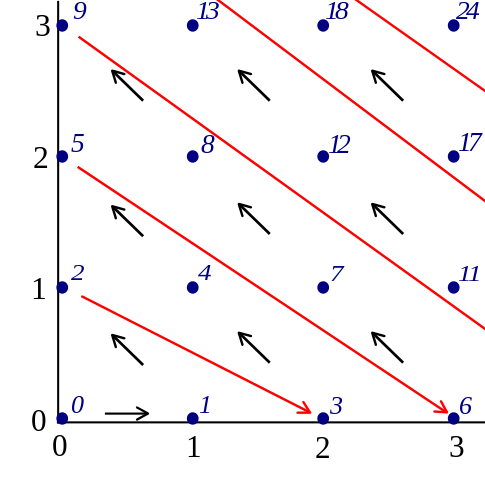
\includegraphics[width=0.4\linewidth]{fig/pairing_natural.png}
    \caption{一种遍历集合$P$中元素的路径}\label{fig:pairing_natural}
\end{figure}

在图~\ref{fig:pairing_natural}~中,我们从原点$\left( 0,0 \right) $开始,沿着箭头
前进,最终途径了所有$P$中元素对应的点。在图中你可以见到,每一个我们到访的节点旁
边都标注了一个自然数,这便是集合$P$中元素的次序。依照这个次序,我们就可以数出所
有集合$P$中的元素,从而说明它是一个无限可数集。

把集合$P$替换为正有理数集合$\left\{\left. \dfrac{a}{b}\,\right|\, a\in 
\mathbb{N},\,b\in\mathbb{N}^\ast \right\} $,那我们同样可以用类似的方法说明
它是一个无限可数集。再根据和$\mathbb{Z}$类似的方法,我们可以说明:

\begin{rawthm}
    自然数集$\mathbb{N}$、正整数集$\mathbb{N}^\ast$、整数集$\mathbb{Z}$和有理数
    集$\mathbb{Q}$四者是等势的。
\end{rawthm}

\subsubsection{$\mathbb{N}$与$\mathbb{R}$不等势:康托尔对角线证明}

1891年,格奥尔格·康托尔(Georg Cantor)提出了\textbf{对角线证明}\index{对角线证
明},证明了实数集是\textbf{不可数集}。也就是说,实数集与有理数集不等势,且实数集
的势大于有理数集。

到目前为止,我们只证明过(至少尝试说明过)集合等势——找到一个一一对应。但如何证明
集合不等势呢?

要证明两个集合不等势,我们要证明两个集合间\emph{不存在}一一对应。也就是说,
\emph{对于任意}我们尝试建立的两个集合间的对应关系$f$,$f$\emph{总不是}一个一一对
应。

显然,尝试找到所有可能的对应关系,并逐个证明它们不是一一对应的做法是不现实的。一
种常见的证明思路是使用反证法。%(我们将在第??章提到) TODO:

在证明中,康托尔研究了自然数集与闭区间$\left( 0,1\right) $。由于后者与实数集等势,
只要证明闭区间的势比自然数集的大就可以说明实数集和自然数集的关系了。康托尔的证明
思路如下。

我们假设$\left( 0,1 \right) $是一个无限可数集。并且我们知道,这个区间内的每一个
数都可以用小数形式表达。

既然这个闭区间是可数的,那我们就将其按照规律列出:

\begin{table}[h]
    \centering
    \caption{假设的一种对应关系}\label{tbl:cantor_diagonal}
    \begin{tabular}{r|l}
        $\mathbb{N}$& $\left( 0,1 \right) $\\
        \hline
        0 & $0.24723159\ldots $\\
        1 & $0.12749325\ldots $\\
        2 & $0.35723957\ldots $\\
        3 & $0.58923933\ldots $\\
        4 & $0.93910272\ldots $\\
        5 & $0.44865920\ldots $\\
        $\vdots$ & $\vdots$
    \end{tabular}
\end{table}

根据我们的假设,表~\ref{tbl:cantor_diagonal}~的左边有所有的自然数,右边则有所有
$\left( 0,1 \right) $中的实数。由于这些实数很有可能是无理数,所以表中都以无限小数
的形式列出(可以把有限小数看成最后有无限个0的无限小数)。

然而,我们说,我们总可以找到(构造出)一个新的数$r$,它不可能出现在表~\ref{tbl:cantor_diagonal}~%
的右边。下面是它的构造方法。

我们先从表中构建一个数字$r_{0}$。我们考虑表~\ref{tbl:cantor_diagonal}~中自然数0
所对应的数(第一个数),取其小数点后第一位数来当我们构造的$r_{0}$小数点后的第一位;
取表中自然数1所对应的数(第二个数)小数点后的第二位,来当$r_{0}$小数点后的第二位;
以此类推,$r_{0}$小数点后第$n$位数总是表~\ref{tbl:cantor_diagonal}~中自然数$n-1$
所对应的实数小数点后的第$n$位,如表~\ref{tbl:cantor_diagonal_maker0}~所示。其中
$r_{0}$所用到的数字用粗体指出。

\begin{table}[h]
    \centering
    \caption{$r_{0}$的构造过程}\label{tbl:cantor_diagonal_maker0}
    \begin{tabular}{r|l}
        $\mathbb{N}$& $\left( 0,1 \right) $\\
        \hline
        0 & $0.\mathbf{2}4723159\ldots $\\
        1 & $0.1\mathbf{2}749325\ldots $\\
        2 & $0.35\mathbf{7}23957\ldots $\\
        3 & $0.589\mathbf{2}3933\ldots $\\
        4 & $0.9391\mathbf{0}272\ldots $\\
        5 & $0.44865\mathbf{9}20\ldots $\\
        $\vdots$ & $\vdots$
    \end{tabular}
\end{table}

这样我们便构造出了
\[
    r_{0}=0.227209\ldots 
\]
接下来是关键的一步,我们将$r_{0}$小数点后的\emph{每一位数都加1}(如果这一位数是9,
那就变成0),把新的数记作$r$。这一步的目的是让$r$小数点后的每一位都与$r_{0}$不同。
我们有:
\[
    r=0.338310\ldots 
\]

那么我们说,这样构造出的$r$\emph{不可能}出现在表~\ref{tbl:cantor_diagonal}~的右
边。也就是说,根据表~\ref{tbl:cantor_diagonal}~的对应关系,不可能有自然数$n$对应
到我们构造出的$r$。

如何证明$n$不存在呢?依然利用反证法。首先,$n$总不可能是0,因为表中0所对应的实数
小数点后的第一位数就与$r$小数点后的第一位数不同;$n$也不可能是1,因为1所对应的实
数小数点后的第二位数与$r$的不同;$n$同样不可能是2,因为2所对应的实数小数点后的第
三位数与$r$的不同……

事实上,对于任意的自然数$k$,$k$在表中所对应的实数(不妨记作$p_k$)小数点后的第
$k+1$位数总与$r$小数点后的第$k+1$位数不同。因为根据$r$的构造过程,$p_k$小数点后
的第$k+1$位数总是和$r_{0}$小数点后的第$k+1$位数相同。但是我们构造中“逐位加1”的操
作保证了$r$小数点后的第$k+1$位数和$r_{0}$的总不同,从而和$p_k$的总不同。

既然$r$与表~\ref{tbl:cantor_diagonal}~右边的每一个数都至少有一位是不同的,那么
$r$显然不会出现在表~\ref{tbl:cantor_diagonal}~的右边了。

这样我们就证明了,一开始的假设是错误的,即\textbf{$\left( 0,1 \right) $不是一个
无限可数集。}对于任意我们尝试建立的对应关系(比如表~\ref{tbl:cantor_diagonal}~那
样),我们总能在$\left( 0,1 \right) $中找到尚未被对应的元素$r$。从而说明,
$\left( 0,1 \right) $与$\mathbb{N}$不等势,且前者的势大于后者。从而我们证明了:

\begin{rawthm}
    $\mathbb{R}$的势大于$\mathbb{N}$,它是一个不可数集。
\end{rawthm}

现在你对于证明集合不等势有了一些认识,请你尝试证明以下命题。

\begin{rawprp}[2024台州二模19题改]
    有理数集$\mathbb{N}$与其幂集$\mathcal{P}(\mathbb{N})$不等势。    
\end{rawprp}


